

\documentclass{pracalicmgr2021}
\usepackage{chngcntr}
%\counterwithout{figure}{chapter}
\counterwithout{table}{chapter}
\counterwithout{equation}{chapter}
\usepackage{polski}
\usepackage[utf8]{inputenc}
\usepackage{indentfirst}
\usepackage{graphicx} 
\bibliographystyle{unsrt}
\usepackage{notoccite}

\author{Mikołaj Boroński}

\nralbumu{418365}

\title{Classification of signals from gravitational wave detectors using spiking neural networks}

\tytulang{???}

\kierunek{Zastosowania Fizyki w Biologii i Medycynie}

\specjalnosc{Neuroinformatyka}

\opiekun{dr hab. inż. Piotr Gawron \\ AstroCeNT, Centrum Astronomiczne im. Mikołaja Kopernika PAN}

%\dziedzina{13.200}
%\dziedzina{13.2 Fizyka}

\date{czerwiec 2022}

\keywords{fale grawitacyjne, klasyfikacja, sieci pulsujące}

\begin{document}


    \maketitle
    \let\cleardoublepage\clearpage
    
    \begin{abstract}
    Streszczenie pracy licencjackiej
    \end{abstract}

    \tableofcontents

    \chapter{Wprowadzenie}
    \section{Stan rozwoju}
    Pojawienie się relatywnie szybkich i dających dobre rezultaty modeli generatywnych (DALL-E, Stable Diffusion), rozwój dużych modeli językowych (LLM), jak na przykład: GPT-4\cite{gpt1}, LLaMA\cite{llama1} oraz ich wersji konwersacyjnych (Chat-GPT\cite{gpt2}) spowodowało prawdziwy wybuch zainteresowania rozwojem sieci głębokich. Sam dostęp do modeli jest jednak udostępniany najczęściej w formie API\cite{gpt3} lub przez aplikację webową\cite{gpt4}, a sam proces uczenia tak dużych sieci jest zbyt kosztowny dla środowiska akademickiego lub mniejszych, gorzej finansowanych podmiotów.
    
    Taki stan rzeczy powodował obawy o zmonopolizowanie dostępu, jak i rozwoju tej technologii, niemożliwość przeprowadzania reprodukowalnych badań i podobne. Sytuacja uległa częściowej poprawie po wycieku wag LLaMA\cite{llama2}. Społeczność open-source w krótkim czasie dokonała szeregu interesujących odkryć, przykładowo: duże modele językowe mogą być dotrenowane przy użyciu relatywnie małych środków\cite{alpaca1}, implementacja C++ pozwalała na uruchamianie inferencji nawet na telefonach komórkowych\cite{llamacpp1}.
    
    Rozwój nie dotyczy jednak tylko tych dwóch kategorii, znaczące postępy poczyniono także w generowaniu wideo\cite{jakis_model_video}, autonomicznych pojazdach\cite{coś_tesla_lub_waymo}, robotyce(?) oraz estymatach 2D-3D\cite{nerf}. Szeregi czasowe chyba nic od daaaaaaaaawna? To może plus być dla SNN.
    
    \section{Problemy}

    Jednym z głównych motorów napędowych ostatnich przełomów jest wzrastająca niemal eksponencjalnie liczba parametrów sieci. 

    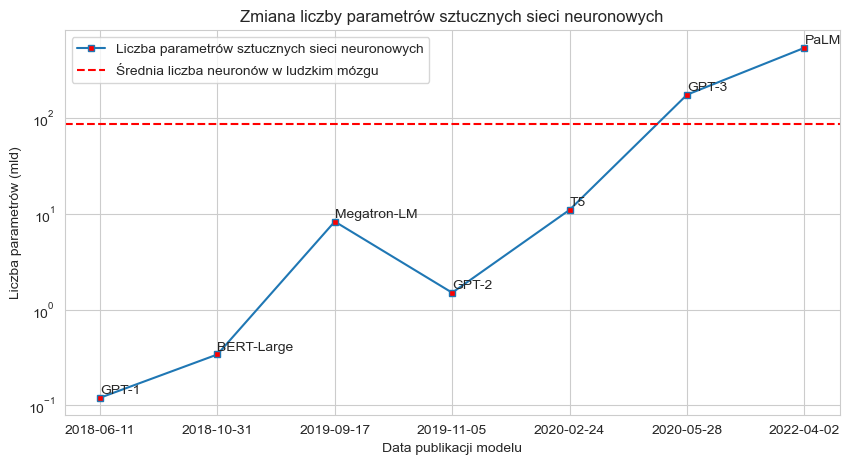
\includegraphics[width=\textwidth]{n_params.png}
    Kompilacja źródeł własna    
    
    - problem trenowania
    - problem inferencji w słabszych urządzeniach, łaziki/auta/cośtam
    - ile energii gpt3, llama
    - liczba parametrow i energii vs mozg 
    - architektura von neumanna i ograniczenia
    
    Above wouldn't be possible without increasing the number of learnable parameters. The StarCraft 2 playing model AlphaStar has 139-milion learnable parameters, image generating model DALL·E 2 tops it with 3.5-billion, but all are being dwarved by language processing models like GPT--3 at 176-billion and Megatron-Turing NLG 530B at 530-billion\cite{alphastar, dalle, gpt, megatron}. This way we can clearly see that more complicated tasks call for a higher number of parameters. Training those models wouldn't be a problem, if not for the earth's limited resources. It takes around 190,000 kWh to train GPT--3 alone\cite{energy}. 
    
    \section{The problem of energy efficiency in von Neumann architecture}
    
    \section{Spiking Neural Networks as a natural step forward}
    
    \section{In pursuit of consciousness}
    
    \section{Overwhelming amounts of data}
    
    
    \chapter{Teoria}
    \section{Overview}
    
    \section{Spiking Neurons}
    
    \section{Input encoding}
    
    \section{Output decoding}
    
    \section{Training and learning rules}
    
    
    \chapter{??? - Istota problemu}
    \section{Overview}
    
    \section{Detectors}
    
    
    \chapter{??? - jakas analiza}
    \section{Data overview}
    
    \section{Data preparation}
    
    \section{Network architecture}
    
    \section{Results -- params1}
    
    \section{Results -- params2}
    
    \section{Results -- params3}
    
    
    \chapter{Podsumowanie}

\bibliographystyle{plain}
\bibliography{bibliografia}
\end{document}

